\documentclass[10pt]{beamer}

\usetheme{metropolis}
\usepackage{appendixnumberbeamer}

\usepackage{booktabs}
\usepackage{multirow}
\usepackage[scale=2]{ccicons}

\usepackage{pgfplots}
\usepgfplotslibrary{dateplot}

\usepackage{xspace}
\newcommand{\themename}{\textbf{\textsc{metropolis}}\xspace}
\usepackage{tabularx}

\usepackage[utf8]{inputenc}
\usepackage[brazilian]{babel}

\usepackage{blindtext}
\setbeamercolor{background canvas}{bg=white}

\title{}
\subtitle{Uso de Redes de Função de Base Radial e Cadeias de Markov para detecção online de mudanças de conceito em fluxos contínuos de dados}
\date{}
\author{\textbf{Discente:} Ruivaldo Neto \newline \textbf{Orientador:} Ricardo Rios}
\institute{Universidade Federal da Bahia \newline Departamento de Ciência da Computação \newline Programa de Pós-Graduação em Ciência da Computação \newline\newline Contato: rneto@rneto.dev \newline\newline 16 de Dezembro de 2019}

\titlegraphic{%
  \begin{picture}(0,0)
    \put(330, 28){\makebox(0,0)[rt]{
\includegraphics[scale=0.25]{logo.png}}}
  \end{picture}
}

\begin{document}

\maketitle

\begin{frame}{Roteiro}
  \setbeamertemplate{section in toc}[sections numbered]
  \begin{minipage}{\textwidth}
    \tableofcontents
  \end{minipage}
\end{frame}

\section{Introdução}

\begin{frame}{Introdução}
    \begin{itemize}
        \item<1 -> Avanços tecnológicos recentes contribuiram para um aumento exponencial no volume de dados produzidos por sistemas computacionais \cite{idc_report}.
        \item<2 -> Parte significativa dos dados é produzida atráves de \alert{Fluxos Contínuos de Dados (FCDs)}: sequências \alert{ininterruptas} e \alert{potencialmente infinitas} de eventos \cite{Aggarwal:2006:DSM:1196418}.
        \item<3 -> FCDs estão presentes em diversos domínios de aplicação:
        \begin{itemize}
            \item Monitoramento de tráfico;
            \item Gestão de redes de telecomunicação;
            \item Análise do Mercado Financeiro;
            \item Detecção de intrusos.
        \end{itemize}
      \end{itemize}
\end{frame}

\begin{frame}{Introdução}
    \begin{itemize}
        \item<1 -> Técnicas de \alert{Aprendizado de Máquina (AM)} têm sido aplicadas para extrair informações úteis de grandes conjuntos de dados.
        \item<2 -> Cenários com FCDs limitam a aplicação de técnicas de AM, pois impõem restrições de tempo de resposta, de uso dos recursos computacionais e apresentam comportamento \alert{não estacionário}.
        \item<3 -> Em cenários não estacionários, o contexto do processo gerador e/ou a distribuição dos dados podem sofrer alterações (\alert{mudanças de conceito}) ao longo do tempo.
        \item<4 -> A ocorrência de \alert{mudanças de conceito} (\textit{concept drifts}) pode impactar a acurácia da técnica aplicada.
      \end{itemize}
\end{frame}

\begin{frame}{Introdução}
    \begin{itemize}
        \item<1 -> A atualização periódica de modelos, apesar de computacionalmente ineficiente, foi utilizada como estratégia para mitigar a perda de acurácia causada por tais mudanças.
        \item<2 -> Visando obter soluções computacionalmente eficientes e com maior precisão, pesquisadores propuseram novos métodos de detecção de mudança de conceito baseados em monitoramento.
      \end{itemize}
\end{frame}


\begin{frame}{Introdução}
    \begin{itemize}
        \item<1 -> Entretanto, os métodos disponíveis na literatura ainda apresentam limitações ao serem aplicados em cenários com FCDs \cite{Aggarwal:2006:DSM:1196418}:
        \begin{itemize}
            \item<2 -> Necessidade de rotulação;
            \item<2 -> Eficiência computacional (tempo de resposta e uso de recursos).
        \end{itemize}
      \end{itemize}
\end{frame}

\begin{frame}{Introdução}
    \begin{itemize}
        \item<1 -> Visando superar essas limitações, este trabalho propõe um novo método de detecção de mudanças de conceito baseado em \alert{Redes de Função de Base Radial (redes RBF) e Cadeias de Markov}, denominado \textbf{\alert{RBFChain}};
        \item<2 -> O método proposto se diferencia por detectar mudanças em tempo de execução, de forma computacionalmente eficiente e independente de rótulos.
    \end{itemize}
\end{frame}

\section{Fundamentação Teórica}

\begin{frame}{Fluxos Contínuos de Dados e Aprendizado de Máquina}
    \begin{itemize}
        \item<1 -> \alert{Fluxos Contínuos de Dados (FCDs)} são sequências ininterruptas e potencialmente infinitas de eventos \cite{Aggarwal:2006:DSM:1196418}.
        \item<2 -> Não podem ser armazenados em sua totalidade e, por serem de alta frequência, devem ser analisados em tempo real.
        \item<3 -> Algoritmos supervisionados \cite{Domingos:2000:MHD:347090.347107, Bifet:2013:EDS:2480362.2480516, Wang:2003:MCD:956750.956778, Aggarwal:2004:DCD:1014052.1014110, Gama:2003:ADT:956750.956813} e não-supervisionados \cite{Aggarwal:2003:FCE:1315451.1315460, Ackermann:2012:SCA:2133803.2184450, Kranen:2011:CIM:2134350.2134352} da área de AM foram adaptados para atenderem a essas restrições.
        \item<4 -> Contudo, essas especializações não tratam a ocorrência de \alert{mudanças de conceito}.
      \end{itemize}
\end{frame}

\begin{frame}{Mudança de Conceito}
    \begin{itemize}
        \item<1 -> A Teoria Bayesiana de Decisão \cite{Duda:2000:PC:954544} é comumente utilizada para descrever a tarefa de classificação e pode ser utilizada para formalizar a noção de \alert{mudança de conceito}.
        \item<2 -> Considerando que $p_{t_0}$ e $p_{t_1}$ denotam as distribuições de probabilidades conjuntas nos instantes $t_0$ e $t_1$, é possível afirmar que há mudança de conceito entre os instantes $t_0$ e $t_1$ se:
        \begin{equation} \label{eq:3}
            {\exists}X : p_{t_0}(X, c) \ne p_{t_1}(X, c)
        \end{equation}
        \item<3 -> Um conjunto de dados possui resultados esperados legítimos em $t_0$, mas este mesmo conjunto passa a ter resultados esperados diferentes, também legítimos, em $t_1$ \cite{Kolter:2007:DWM:1314498.1390333}.
    \end{itemize}
\end{frame}

\begin{frame}{Mudança de Conceito}
    \begin{itemize}
        \item<1 -> As mudanças de conceito podem ser categorizadas como \alert{Virtuais} ou \alert{Reais} \cite{Gama:2014:SCD:2597757.2523813}:
        \begin{itemize}
        \item<2 -> \alert{Mudanças Virtuais} são causadas por alterações na probabilidade a priori das classes, $P(c)$, e não alteram os conceitos-alvo.
        \item<3 -> \alert{Mudanças Reais} surgem a partir de alterações na probabilidade a posteriori, $p(c|X)$, e modificam os resultados esperados.
        \end{itemize}
    \end{itemize}
\end{frame}

\begin{frame}{Mudança de Conceito}
\begin{figure}[H]
    \begin{center}
        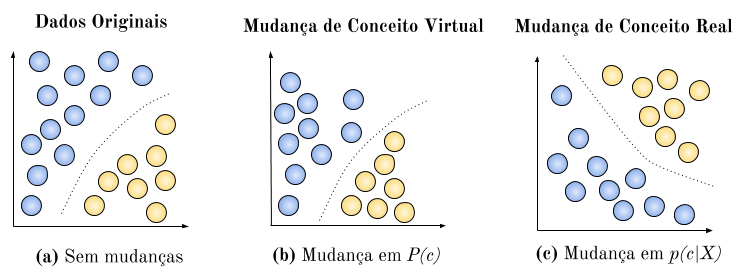
\includegraphics[scale=0.5]{imagens/concept_drift.png}
        \caption{Mudança de Conceito Virtual vs. Mudança de Conceito Real}
        \label{fig:real_and_virtual_concept_drift}
    \end{center}
\end{figure}
\end{frame}

\begin{frame}{Mudança de Conceito}
    \begin{itemize}
        \item<1 -> As mudanças de conceito podem ocorrer de forma \alert{abrupta}, \alert{gradual}, \alert{incremental} ou \alert{recorrente} \cite{Zliobaite:2010}.
    \end{itemize}
    \begin{figure}[H]
        \begin{center}
            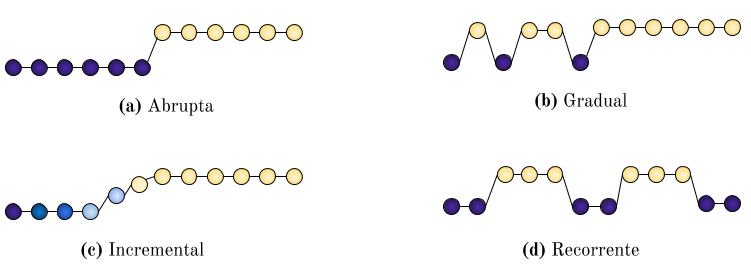
\includegraphics[scale=0.5]{imagens/concept_drift_patterns.png}
            \caption{Padrões de ocorrência de Mudanças de Conceito}
            \label{fig:concept_drift_patterns}
        \end{center}
    \end{figure}
\end{frame}

\begin{frame}{Algoritmos para Detecção de Mudança de Conceito}
    \begin{itemize}
        \item<1 -> Os algoritmos para Detecção de Mudanças de Conceito se dividem em duas categorias, conforme a necessidade de rotulação dos dados \cite{Zliobaite:2010}:
        \begin{itemize}
        \item<2 -> \alert{Explícitos/Supervisionados}: Dependem da rotulação dos dados, pois realizam a detecção a partir do monitoramento de medidas de performance como taxa de erro e acurácia.
        \item<3 -> \alert{Implícitos/Não Supervisionados}: Independem da rotulação dos dados, realizando a detecção através do monitoramento de características dos próprios dados ou de indicadores produzidos pelas técnicas de aprendizado aplicadas.
        \end{itemize}
    \end{itemize}
\end{frame}

\begin{frame}{Ferramenta: MOA}
    \begin{itemize}
        \item<1 -> Principal framework para mineração de dados em fluxos contínuos.
        \item<1 -> Permite implementar e validar novos métodos de detecção de mudança de conceito de forma trivial.
    \end{itemize}
    \begin{figure}[H]
        \begin{center}
            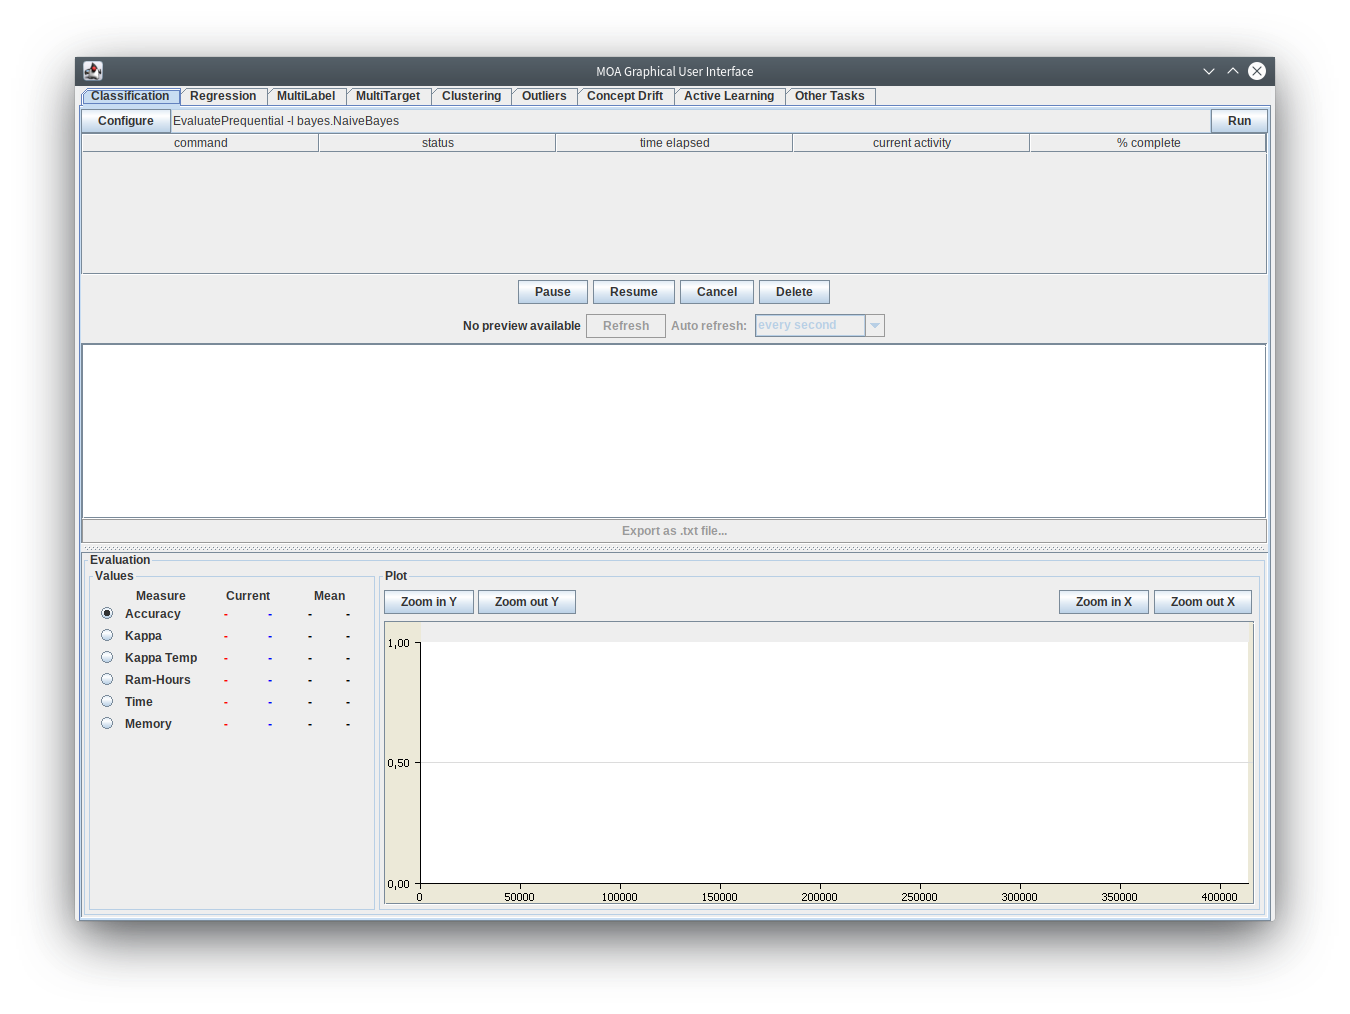
\includegraphics[scale=0.2]{imagens/moa.png}
            \caption{MOA - Tela Inicial}
            \label{fig:moa}
        \end{center}
    \end{figure}
\end{frame}

\begin{frame}{Mudança de Conceito - RBFChain}
    \begin{itemize}
        \item<1 -> O método proposto neste trabalho é capaz de identificar mudanças \alert{sob qualquer padrão de ocorrência};
        \item<2 -> Por ser independente de rótulos, considera todas mudanças identificadas como \alert{mudanças reais};
        \item<3 -> Implementado e validado através da plataforma MOA.
    \end{itemize}
\end{frame}

\begin{frame}{Redes de Função de Base Radial}
    \begin{itemize}
        \item<1 -> \alert{Redes de Função de Base Radial} são redes neurais cujo principal diferencial é a forma de ativação, realizada através do cálculo da distância entre o dado e um centro definido \cite{Braga:RedesNeuraisTeoriaAplicacoes}.
        \item<2 -> A arquitetura de uma rede RBF, em sua forma mais básica, envolve três camadas:
        \begin{itemize}
            \item<3 -> \alert{Entrada}: Recepciona os dados e encaminha para camada intermediária.
            \item<4 -> \alert{Intermediária}: Composta por funções de ativação de base radial que atuam como neurônios.
            \item<5 -> \alert{Saída}: Pondera os resultados da camada intermediária, agregando-os linearmente para compor a resposta final da rede.
        \end{itemize}
        \item<6 -> Na literatura, as funções Gaussianas são as funções de ativação mais usuais em redes RBF.
      \end{itemize}
\end{frame}

\begin{frame}{Redes de Função de Base Radial}
    \begin{figure}[H]
    \begin{center}
        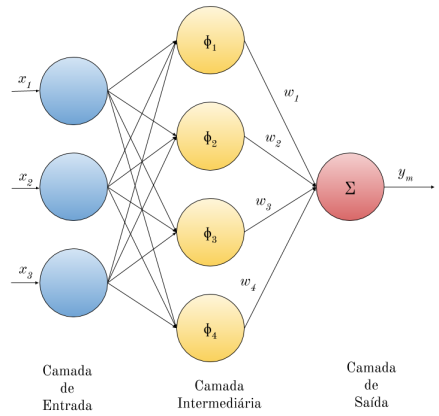
\includegraphics[scale=0.6]{imagens/rbf_arq.png}
        \caption{Arquitetura RBF}
        \label{fig:rbg_arq}
    \end{center}
    \end{figure}
\end{frame}

\begin{frame}{Redes de Função de Base Radial}
    \begin{itemize}
        \item<1 -> O RBFChain utilizar uma rede RBF adaptada, composta apenas pelas camadas inicial e intermediária;
        \item<2 -> O processo de ativação realizado na camada intermediária produz, implicitamente, grupos a partir das observações recebidas ao longo do tempo;
        \item<3 -> Mudanças de conceito podem ser identificadas quando o grupo ativo deste agrupamento é alterado.
      \end{itemize}
\end{frame}


\section{RBFChain}

\begin{frame}{Lorem Ipsum}
    \begin{itemize}
        \item<1 -> A:
        \begin{itemize}
            \item<2 -> A1;
            \item<2 -> A2.
        \end{itemize}
        \item<3 -> B
      \end{itemize}
\end{frame}

\section{Experimentos}

\begin{frame}{Lorem Ipsum}
    \begin{itemize}
        \item<1 -> A:
        \begin{itemize}
            \item<2 -> A1;
            \item<2 -> A2.
        \end{itemize}
        \item<3 -> B
      \end{itemize}
\end{frame}

\section{Conclusões e Trabalhos Futuros}

\begin{frame}{Lorem Ipsum}
    \begin{itemize}
        \item<1 -> A:
        \begin{itemize}
            \item<2 -> A1;
            \item<2 -> A2.
        \end{itemize}
        \item<3 -> B
      \end{itemize}
\end{frame}

\begin{frame}[allowframebreaks]{Referências}

  \bibliography{slides}
  \bibliographystyle{abbrv}

\end{frame}

\end{document}
